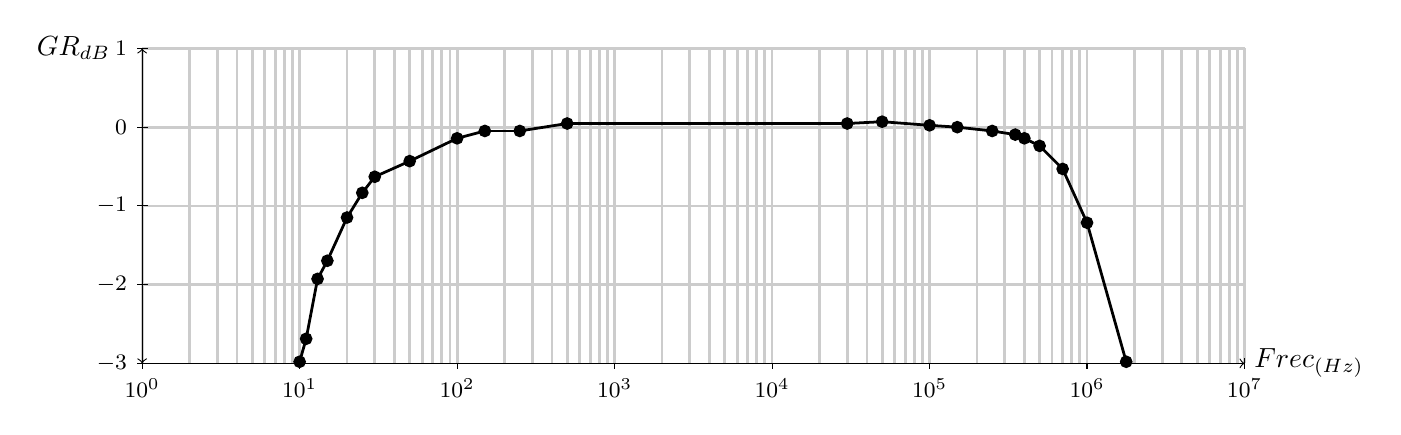
\begin{tikzpicture}[scale=1]

    \def\scalya{3}
    \def\scaly{1}
    \def\scalx{2}
    \def\scalxa{3}
    
    %datosLineaA
    \coordinate (a1) at ({\scalx*log10(10)}, {\scaly*(20*log10(5.28/7.44) + \scalya)});
    \coordinate (a2) at ({\scalx*log10(11)}, {\scaly*(20*log10(5.46/7.44) + \scalya)});
    \coordinate (a3) at ({\scalx*log10(13)}, {\scaly*(20*log10(5.96/7.44) + \scalya)});
    \coordinate (a4) at ({\scalx*log10(15)}, {\scaly*(20*log10(6.12/7.44) + \scalya)});
    \coordinate (a5) at ({\scalx*log10(20)}, {\scaly*(20*log10(6.52/7.44) + \scalya)});
    \coordinate (a6) at ({\scalx*log10(25)}, {\scaly*(20*log10(6.76/7.44) + \scalya)});
    \coordinate (a7) at ({\scalx*log10(30)}, {\scaly*(20*log10(6.92/7.44) + \scalya)});
    \coordinate (a8) at ({\scalx*log10(50)}, {\scaly*(20*log10(7.08/7.44) + \scalya)});
    \coordinate (a9) at ({\scalx*log10(100)}, {\scaly*(20*log10(7.32/7.44) + \scalya)});
    \coordinate (a10) at ({\scalx*log10(150)}, {\scaly*(20*log10(7.40/7.44) + \scalya)});
    \coordinate (a11) at ({\scalx*log10(250)}, {\scaly*(20*log10(7.40/7.44) + \scalya)});
    \coordinate (a12) at ({\scalx*log10(500)}, {\scaly*(20*log10(7.48/7.44) + \scalya)});
    \coordinate (a13) at ({\scalx*(log10(30) + \scalxa)}, {\scaly*(20*log10(7.48/7.44) + \scalya)});
    \coordinate (a14) at ({\scalx*(log10(50) + \scalxa)}, {\scaly*(20*log10(7.50/7.44) + \scalya)});
    \coordinate (a15) at ({\scalx*(log10(100) + \scalxa)}, {\scaly*(20*log10(7.46/7.44) + \scalya)});
    \coordinate (a16) at ({\scalx*(log10(150) + \scalxa)}, {\scaly*(20*log10(7.44/7.44) + \scalya)});
    \coordinate (a17) at ({\scalx*(log10(250) + \scalxa)}, {\scaly*(20*log10(7.40/7.44) + \scalya)});
    \coordinate (a18) at ({\scalx*(log10(350) + \scalxa)}, {\scaly*(20*log10(7.36/7.44) + \scalya)});
    \coordinate (a19) at ({\scalx*(log10(400) + \scalxa)}, {\scaly*(20*log10(7.32/7.44) + \scalya)});
    \coordinate (a20) at ({\scalx*(log10(500) + \scalxa)}, {\scaly*(20*log10(7.24/7.44) + \scalya)});
    \coordinate (a21) at ({\scalx*(log10(700) + \scalxa)}, {\scaly*(20*log10(7.00/7.44) + \scalya)});
    \coordinate (a22) at ({\scalx*(log10(1000) + \scalxa)}, {\scaly*(20*log10(6.47/7.44) + \scalya)});
    \coordinate (a23) at ({\scalx*(log10(1500) + \scalxa)}, {\scaly*(20*log10(5.66/7.44) + \scalya)});
    \coordinate (a23) at ({\scalx*(log10(1773) + \scalxa)}, {\scaly*(20*log10(5.28/7.44) + \scalya)});

    
    %Ejex
    \foreach \x [evaluate={\a=int(\x+1)}]in {0,...,6}{
    \foreach \y in {1,...,10}
        \draw[line width=1pt,gray!40] ({(\x+log10(\y))*\scalx},0)--({(\x+log10(\y))*\scalx},4);
        \draw[shift={(\a*\scalx,0)}] (0pt,2pt) -- (0pt,-2pt) node[below] {\footnotesize $10^\a$};
    }
    \draw[shift={(0,0)}] (0pt,2pt) -- (0pt,-2pt) node[below] {\footnotesize $10^0$};
    \draw[->] (0,0)--(14,0) node[right] {$Frec_{(Hz)}$};
    
    %Ejey
    \foreach \y [evaluate={\a=int(\y-3)}] in {1,...,4}{
        \draw[line width=1pt,gray!40] (0,\y*\scaly)--(14,\y*\scaly);
        \draw[shift={(0,\y*\scaly)}] (2pt,0pt) -- (-2pt,0pt) node [left] {\footnotesize $\a$};
    }
   \draw[shift={(0,0)}] (2pt,0pt) -- (-2pt,0pt) node [left] {\footnotesize $-3$};
   \draw[<->] (0,0)--(0,4) node[left=8pt]{$GR_{dB}$};
   
   
    %Linea A
    \foreach \x  in {1,...,23}{
        \draw[line width=1.5pt,fill=black] (a\x) circle(1.5pt);
   }
   \foreach \x [evaluate={\y=int(\x+1);}] in {1,...,22}{
        \draw[line width=1pt,black] (a\x) -- (a\y);
   }
   
\end{tikzpicture}